% !TeX root = ../libro.tex
% !TeX encoding = utf8

\chapter{Red Neuronal}
\section{El problema de clasificar una imagen.}

Cuando observamos una imagen, podemos localizar varios elementos a partir de los cuáles esta se encuentra compuesta con tan sólo un vistazo. Sin embargo, para un ordenador no se trata de algo tan sencillo puesto que sólo es capaz de ver un gran conjunto de números que no tienen por qué tener relación alguna entre sí.\newline

\begin{figure}[htpb]
  \centering
  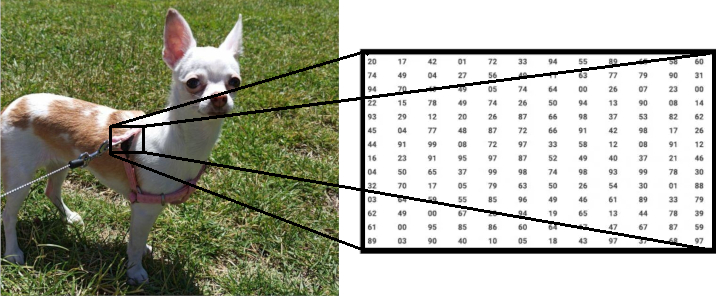
\includegraphics[width=0.8\textwidth]{blanquita}
  \caption{Cómo un ordenador ve una imagen}
  \label{fig:blanquita}
\end{figure}

Idealmente, en esta imagen desearíamos que fuera capaz de identificar que se trata de un perro, en concreto de un chiguagua, de pelaje blanco y manchas color café que se encuentra sobre un césped. Estos poquitos datos que para nosotros parecen tan triviales necesitan de horas y horas de computación para ser obtenidos a partir de una imagen cualquiera.\newline

Dejamos todos estos detalles, a los cuales esperamos poder llegar en un futuro no muy lejano, y simplificamos el problema a tener un conjunto de etiquetas y buscar con cuál de todas ellas tiene mayor relación nuestra imagen.\newline

Una primera idea, sería utilizar utilizar \emph{$k$-Nearest Neighbor Classifier}, en adelante $k$-NN. Este clasificador consiste en que para cada etiqueta se correspondan $k$ imágenes y consideraremos como etiqueta idónea para nuestra clasificación aquella cuya distancia, siendo Manhattan y Euclídea las más comunes, entre los píxeles con nuestra imagen sea menor. Nos encontramos con que el tiempo de entrenamiento de nuestro clasificador sería ínfimo en comparación con el tiempo de clasificación, si bien se pueden hacer diversas mejoras que cambien estos hechos. \newline

De esta sencilla propuesta, surgen diversos problemas. Al darle mayor importancia al valor concreto de los píxeles, en lugar de a las formas que de las que está compuesta la figura, nos encontramos con que valores como los colores de fondo pueden influir más en la clasificación que los propios píxeles de la figura que queremos clasificar. En el ejemplo de la imagen del chiguagua, si considerásemos las etiquetas verde y perro, tendríamos que por lo general como respuesta el color verde, pese a que estamos más interesados por la mascota en sí. Otro gran problema, sería la baja escalabilidad que nos proporciona esta solución, al incrementarse enormemente el costo computacional de clasificación conforme aumenta el número de etiquetas.\newline

El siguiente paso, es buscar una forma de ``memorizar'' los datos de entrenamiento de forma que no tengamos que estar comparándolos con todos ellos cuando queramos clasificar una imagen. Lo que buscamos es poder valorar de alguna forma la imagen completa y a partir de esta ``puntuación'' conocer qué etiqueta le corresponde mejor a nuestra imagen. De esta forma, veríamos drásticamente reducido el tiempo de clasificación, sacrificando para ello el tiempo de entrenamiento, y podríamos ampliar en varias unidades la cantidad de datos de entrenamiento utilizados, aumentando así la precisión de nuestro clasificador.

\section{Clasificadores Lineales}

Antes de nada, vamos a comenzar contextualizando matemáticamente el entorno en el que nos encontramos. Una vez realizado esto podremos hablar correctamente de los clasificadores lineales y así poder extenderlos naturalmente a los conceptos de Red Neuronal y de Red Neuronal Convolucionada.\newline

Sea $D \in \N$ la dimensión de nuestras imágenes, por lo general el número de píxeles que estas poseen, y $K \in \N$ la cantidad de etiquetas o categorías bajo las cuales pueden ser clasificadas. Siendo $N \in \N$ el número de ejemplos que utilizaremos para entrenar nuestro clasificador, tendremos que para cada dato de entrenamiento $x_i \in \R^D \; i=1,...,N$ le corresponde una etiqueta $y_i \in 1,...,K$ tal que juntos conforman el par $(x_i,y_i)$ de imagen y categoría a la que pertenece.\newline

Para que no sea más fácil de entender este contexto, tomaremos como ejemplo el conjunto de datos CIFAR-10 que consiste en 60000 imágenes RGB de dimensión 32x32 y 10 categorías. De esta forma, tendríamos que $D=32\cdot 32 \cdot 3 = 3072$, $K=10$ y $N=60000$.

\begin{definicion}\label{def:ScoreFunction}
Definiremos \emph{función de puntuación} o \emph{score function} como una función $f:\R^D \to \R^K$ que asigna los píxeles de la imagen sin procesar una serie de puntuaciones para cada etiqueta.
\end{definicion}

Una función de puntuación nos revela la probabilidad que tiene cada imagen de pertenecer a cada una de la distintas etiquetas de las que disponemos. Podemos definir un \emph{clasificador lineal} o \emph{linear classifier} \label{def:LinearClassifier} como aquel que utiliza una función de puntuación lineal, es decir, de la forma:

$$f(x)=W\cdot x+ b\; \; \; W\in M_{K,D}(\R) \;\; b \in \R^K \;\; \forall x\in \R^D$$

Dicho esto, existen diferentes tipos de clasificadores lineales y la principal diferencia entre ellos reside en la función de pérdida que utilicen a la hora de entrenar la red.

\begin{definicion}\label{def:LossFunction}
Una \emph{función de pérdida} o \emph{loss function} es aquella que durante el entrenamiento de un clasificador se encarga de penalizar las etiquetas incorrectas.
\end{definicion}

FIXME: ¿Hablar de SVM, SoftMax y Cross-Entropy?\newline

Llegados a este punto, debemos de explicar cómo funcionan los clasificadores lineales, es decir, cómo estos son entrenados y para qué se emplean las funciones de puntuación y de pérdida. Dado poseemos un conjunto de ejemplos con su correspondiente etiqueta pero desconocemos el valor de los parámetros $W$ y $b$, nuestro objetivo es utilizar dichos datos de entrenamiento para estimar estos valores. \newline

Para ello, comenzamos haciendo una conjetura sobre un posible valor para nuestros parámetros, evaluamos nuestra función de puntuación con todos nuestros datos de entrenamiento y seguidamente utilizamos la función de pérdida para estimar cómo de bien funciona nuestra conjetura. Analizamos los resultados y hacemos una nueva conjetura que los mejore, repitiendo el proceso un número lo suficientemente grande de veces.\newline

Seguidamente, debemos preguntarnos cómo realizamos la nueva conjetura de forma que nos aseguremos tener unos resultados mejores. Hacerlo de forma totalmente aleatoria, repitiéndolo hasta obtener una pérdida lo suficientemente pequeña, no parece una buena idea puesto que es difícil saber cuándo encontraremos una buena respuesta. Entre las distintas técnicas, nos encontramos con las basadas en la \emph{búsqueda aleatoria local} y las que se basan en el \emph{Gradiente Descendiente}, entre otras muchas. Como ejemplo, tomaremos el algoritmo del gradiente descendiente y minimizaremos la función de pérdida para llegar a aquellos pesos que menor error nos den.\newline

FIXME: Enlazar pdfs que expliquen bien cómo funciona el gradiente descendiente y la búsqueda aleatoria local \newline
\lstset{language=Python}
\begin{lstlisting}[frame=single]
while condicion_de_parada :
  weight_grad=evaluate_grad(loss_fun,x,y)
  weight = -step_size*weight_grad

\end{lstlisting}

El código mostrado más arriba se trata de una versión muy simplificada de cómo funcionaría de cómo podríamos implementar el algoritmo, teniendo en cuenta que nosotros mismos podremos modificar la condición de parada de acuerdo a nuestras necesidades y que el valor \emph{step\_size} es algo que podremos fijar de la misma forma, sabiendo que este nos indica cuánto queremos avanzar en la dirección que nos indica el gradiente. FIXME: Enlazar pdfs que expliquen la importancia de estos valores y cómo fijarlos.\newline

FIXME: Añadir implementación en Tensorflow de un clasificador lineal.

\begin{ejemplo}\label{SoftMaxBinary}
Fijemos una etiqueta, $y=0$ por lo que $K=1$. Tendríamos que nuestra función de puntuación sería $f:\R^D \to \R$ donde $W=(w_1,...w_D)\in \R^D$ y $b\in \R$ luego $$f(x)=W\cdot x + b = \sum_{j=1}^D w_j x_j+b.$$ Así mismo, tomamos como función de pérdida $$L(x,f)=-\ln \frac{1}{\sum_{j=1}^D e^{f_j}}=-\ln \frac{1}{\sum_{j=1}^D e^{w_j x_j +b}}=\ln\sum_{j=1}^D e^{w_j x_j +b}$$ que es un caso particular de \emph{Entropía Cruzada} o \emph{Cross-entropy}.\newline

Este clasificador recibe el nombre de \emph{Binary Softmax classifier} o \emph{Binary Logistic Regression classifier}. De esta forma, si consideramos la función probabilística \emph{sigmoide} tendríamos que el minimizar la función de pérdida estaríamos aumentando la probabilidad clasificar correctamente nuestros datos puesto que: $$P(y=0 | x; W)=\sigma (f(x)) = \frac{1}{1+e^{-f(x)}}.$$

\begin{observacion}
Estamos calculando la probabilidad de coincidir o no con una determinada etiqueta, recibe el nombre de binario porque también podríamos considerar que tenemos dos etiquetas y que si no perteneces a una forzosamente perteneces a la otra. Este modelo puede por tanto construirse también utilizando ambas etiquetas y con mejores resultados a la hora de clasificar puesto que durante el entrenamiento la función de pérdida es ligeramente modificada para tener en cuenta la otra etiqueta. En cualquier caso, ambas construcciones siguen la misma interpretación probabilística y, además, tenemos que $P(y=1 | x; W)=1-P(y=0 | x; W)$.
\end{observacion}
\end{ejemplo}

\begin{ejemplo}\label{SVM}
Tomamos como función de pérdida $L(x,f)=\frac{1}{N} \sum_{i=1}^N \sum_{j \neq y_i} \max(0,f_j-f_{y_i} + \Delta)$ donde $\Delta \in \R$ es un parámetro que se suele ajustar utilizando una técnica llamada \emph{validación cruzada} o \emph{cross validation}. Esta función suele recibir el nombre de \emph{hinge loss} y el clasificador lineal es conocido como \emph{Multiclass Suport Vector Machine (SVM)}. Este clasificador "quiere" que la etiqueta correcta para cada imagen tenga una puntuación mayor que las incorrectas por un margen fijo $\Delta$.
\end{ejemplo}
\section{El modelo de una neurona}

Cuando comenzamos planteando nuestro problema buscábamos conseguir clasificar una imagen con una probabilidad de acertar similar o superior a cómo lo haríamos nosotros mismos. Teníamos el problema de que un ordenador no era capaz de pensar o razonar de la misma forma que un ser humano y buscábamos una forma de clasificar esta información a pesar de ello. Es aquí donde nacen los modelos de redes neuronales, en un intento por ser capaces de simular cómo funciona nuestro propio cerebro en nuestros clasificadores y que estos sean capaces de aprender cómo reconocer los distintos elementos de la misma forma que nosotros lo hemos ido haciendo a lo largo de nuestra vida.\newline

\begin{figure}[htpb]
  \centering
  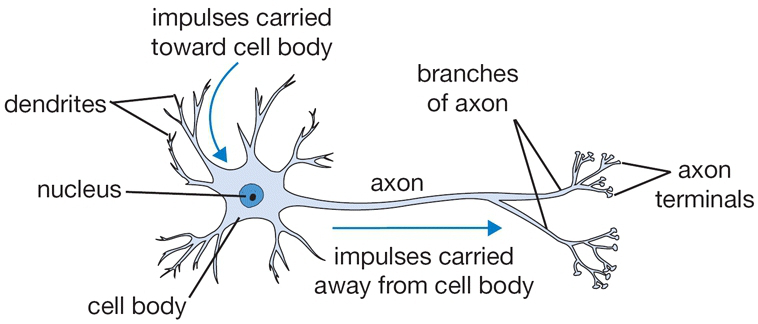
\includegraphics[width=0.45\textwidth]{neuron}
  \vrule
  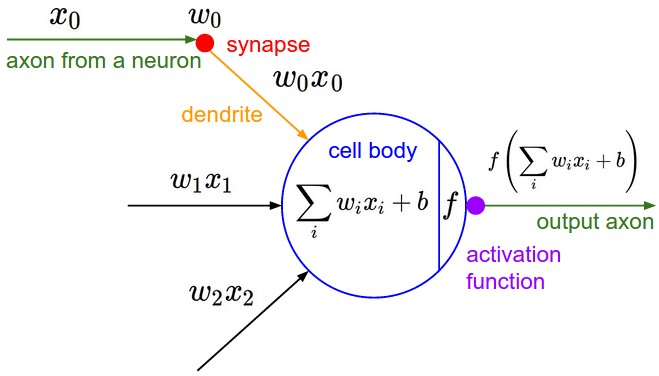
\includegraphics[width=0.45\textwidth]{neuron_model}
  \caption{Comparación entre una neurona biológica (izquierda) y el modelo matemático (derecha) }
  \label{fig:neurona}
\end{figure}

Nuestro cerebro está formado por múltiples neuronas interconectadas entre sí que están constantemente transmitiéndose información y aprendiendo a través de todos los datos que reciben. Si nos fijamos en \ref{fig:neurona} podemos ver que una neurona real esta formada por dentritas que son quienes, a través del proceso de sinapsis, reciben la entrada de información, que es asimilada y transformada por su núcleo antes de ser transmitida a la siguientes neuronas a través de las divisiones de su axón en caso de que supere un cierto umbral y se active.\newline

De esta forma, si consideramos que tenemos $D$ dentritas y que por la $i$-dentrita recibimos el la información $x_i$ con un peso o fuerza de sinapsis $w_i$, tendríamos que nuestro núcleo trabaja con el vector de información $(w_1 x_1,...,w_D x_D)$ que podemos condensar utilizando la norma $||\cdot ||_1$ como $\sum_i w_i x_i $ y sumarle una determinada constante $b$ propia de la neurona. El umbral de activación y la señal enviada al resto de neuronas la representaremos con la \emph{función de activación}\label{def:ActivationFunction} que será una función $f: \R \to \R$. \newline

A continuación, mencionaremos los ejemplos más representativos utilizados como funciones de activación, enlazándolos con lo ya visto anteriormente:

\begin{itemize}
\item \emph{Función sigmoide} $\sigma: \R \to [0,1]$ definida como $\sigma(x)=\frac{1}{1+e^{-x}} $. En este caso, nos encontramos con el ejemplo \ref{SoftMaxBinary} transformado en una neurona cuya función de pérdida utilizada durante el entrenamiento suele ser la misma que en el ejemplo mencionado. Se suele utilizar en la última capa de nuestra red, cuando nuestras imágenes pueden pertenecer a varias clases o etiquetas al mismo tiempo.
\item \emph{Función Softmax} utilizada normalmente en la última capa donde hay tantas neuronas como etiquetas y en el problema de clasificación donde una imagen puede pertenecer únicamente a una sola etiqueta o caso. Se trata de una modificación de función la sigmoide que regulariza la salida para obtener la probabilidad de pertenecer a cada clase como sucesos independientes obteniendo así que la suma de todas las salidas de esta capa sería 1. Aquí, la $i$-neurona tendría función de activación $\sigma_i(x)=\frac{e^{x_i}}{\sum_{j=1}^K e^{x_j}}$ y utilizaría $L(x)=\frac{1}{N}\sum_{i=1}^N -\ln \frac{e^{f_{y_i}}}{\sum_{j=1}^D e^{f_j}}=\frac{1}{N}\sum_{i=1}^N (-{f_{y_i}}+\ln \sum_{j=1}^D e^f_j)$ como función de pérdida para el entrenamiento.
\item \emph{Función ReLU}, cuyo nombre completo sería \emph{Rectified Lineal Unit}. Se suele utilizar en las capas intermedias de nuestra red y utiliza como función de activación $f(x)=\max(0,x)$ que nos recuerda al ejemplo \ref{SVM}.
\item \emph{Función Tanh} se trata de de una centralización de la función sigmoide. $Tanh(x)=2\sigma(x)-1$.
\end{itemize}

\section{La red completa}

Una red red neuronal es un conjunto de neuronas dividas en varias \emph{capas} de forma que las neuronas de una capa pueden estar unidas o no con las neuronas de la capa anterior y de la siguiente formando así un grafo acíclico.\newline

\begin{figure}[htpb]
  \centering
  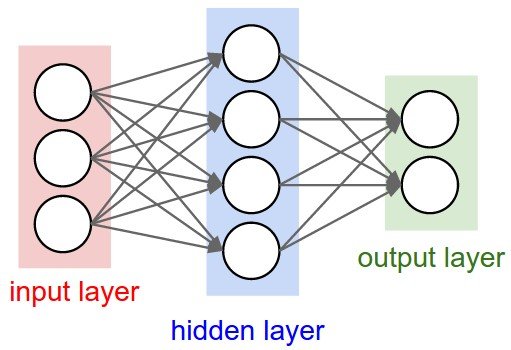
\includegraphics[width=0.4\textwidth]{neural_net}
  \vrule
  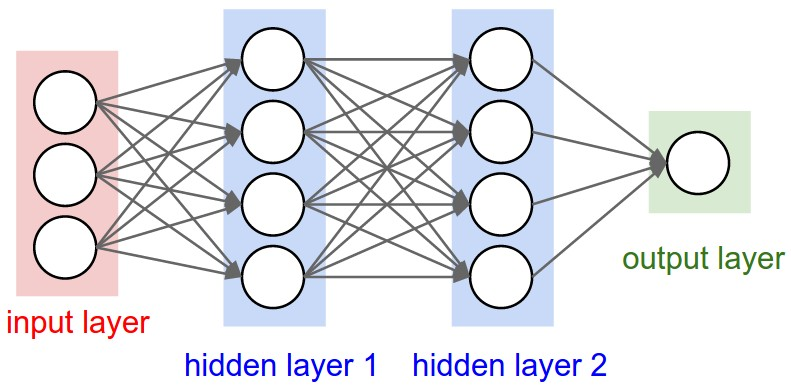
\includegraphics[width=0.5\textwidth]{neural_net2}
  \caption{Ejemplos de redes totalmente conectadas (\emph{fully-connected}) }
  \label{fig:fully-connected}
\end{figure}

La primera capa recibe el nombre de \emph{capa de entrada} que posee $D$ neuronas, es decir, tantas como la dimensión de nuestros datos. Por otro lado tenemos la \emph{capa de salida} con $K$ neuronas, tantas como etiquetas o clases de clasificación tengamos. El resto de neuronas se distribuyen dentro las \emph{capas ocultas} cuya distribución y conexiones dependen del modelo en concreto que queramos desarrollar, quedando a nuestro criterio.\newline

De esta forma, podemos afirmar que una red neuronal es la aplicación sucesiva de funciones de la forma

$$F(x)=\sum_{i=1}^n \alpha_i \sigma(w_i^Tx+b_i) \;\;\; \forall x \in \R^n,$$

donde $w_i\in\R^n,\;\; \alpha_i,b_i\in\R$ serán fijas una vez entrenada la red y $\sigma : \R \to \R$ la función de activación elegida en cada capa.\\

A continuación toca hablar del entrenamiento de la red completa, a los conceptos que ya conocíamos del clasificador lineal \ref{def:LinearClassifier} se añade el concepto de \emph{Backpropagation} o \emph{Propagación hacia atrás de errores} que hace uso de la \emph{regla de la cadena} para, a través de los cálculos locales realizados por cada neurona, obtener la función completa de clasificación. Así, buscamos que las neuronas se auto organicen para ser capaces de localizar patrones similares de forman que sepan cómo reaccionar ante la presencia de ruido o datos incompletos. Esto hace a través de la comunicación de sus valores locales y gradientes entre las distintas neuronas, comenzando por la capa de salida y avanzando hacia atrás. FIXME: Mencionar importancia del Subgradiente para el cálculo del gradiente, al no estar definido para cualquier función. \newline

FIXME: Definir epoch y la validación cruzada

\chapter{Teoremas de Aproximación Universal}
Hasta ahora se ha definido una estructura con una serie de parámetros con la esperanza de poder llegar a resolver el problema planteado. Sin embargo, en ningún momento hemos utilizado ningún resultado que nos asegure que dicha estructura puede llegar a resolver el problema que deseamos. A continuación, mostraremos diversos resultados, con diversos niveles de generalidad, que muestran cómo esta estructura puede llegar a cumplir con lo deseado. Estos resultados se dividen en dos grandes categorías \emph{anchura indeterminada} y \emph{profundidad indeterminada}.

\section{Anchura indeterminada}
\subsection{Geoge Cybenko, 1989}
Cybenko, en \cite{cybenko1989approximation}, demostró la capacidad de aproximación en el caso de anchura indeterminada y profundidad fijada para funciones de activación sigmoidales \autoref{def:sigmoidal}. A partir de esta versión clásica, se logró considerar otras funciones de activación, e incluso, demostrar que era gracias a la arquitectura en sí misma, y no a la función de activación, que las redes neuronales eran aproximadores universales. Aquí mencionaremos la versión del teorema para funciones continuas, pero debemos mencionar que en el mismo artículo se mencionan también versiones para otros espacios de funciones.
\begin{definicion}\label{def:sigmoidal}
Una función $\sigma : \R \to \R$ es \emph{sigmoidal} si $$\lim_{t\to +\infty} \sigma(t)=1 \;\;\;\;\;\;\; \lim_{t\to -\infty} \sigma(t)=0$$
\end{definicion}\\

En adelante, utilizaremos $I_n$ para referirnos al cubo unidad $n$-dimensional, $[0,1]^n$ y para el espacio de las medidas finitas con signo regulares de Borel sobre $I_n$ utilizaremos $M(I_n)$. Además, $C(I_n)$ denotará el espacio de funciones continuas en $I_n$.

\begin{definicion}\label{def:discriminatoria}
Una función $\sigma : \R \to \R$ es \emph{discriminatoria} si para una medida $\mu \in M(I_n)$ con $$\int_{I_n} \sigma(w^Tx+b) d\mu(x)=0$$ para todo $ w\in R^n$ y $b\in\R$ implique que $\mu=0$.
\end{definicion}

\begin{lema}\label{thm:lema-discriminatoria-sigmoidal}
Cualquier función sigmoidal medible y acotada es discriminatoria. En particular, las funciones sigmoidales continuas son discriminatorias.
\end{lema}

\begin{teorema}\label{thm:discriminatoria}
Sea $\sigma$ una función discriminatoria continua. Entonces, las sumas finitas de la forma $$G(x)=\sum_{i=1}^n \alpha_i \sigma(w_i^Tx+b)$$ son densas en $C(I_n)$. En otra palabras, dados $f\in C(I_n)$ y $\varepsilon>0$, existe una suma, $G(x)$, de la forma anterior, para la cual $$|G(x)-f(x)|<\varepsilon \;\;\;\;\; \forall x \in I_n.$$
\end{teorema}
\begin{proof}
\end{proof}
\begin{teorema}\label{thm:sigmoidal}
Sea $\sigma$ una función sigmoidal continua. Entonces, las sumas finitas de la forma $$G(x)=\sum_{i=1}^n \alpha_i \sigma(w_i^Tx+b)$$ son densas en $C(I_n)$. En otra palabras, dados $f\in C(I_n)$ y $\varepsilon>0$, existe una suma, $G(x)$, de la forma anterior, para la cual $$|G(x)-f(x)|<\varepsilon \;\;\;\;\; \forall x \in I_n.$$
\end{teorema}
\begin{proof}
Para esta demostración, se combina \autoref{thm:lema-discriminatoria-sigmoidal} y \autoref{thm:discriminatoria}, notando que las funciones sigmoidales continuas satisfacen las condiciones de este lema.
\end{proof}

\subsection{Kurt Hornik, 1989 y 1991}

En 1898 \cite{HornikEtAl89}, Hornik demostró que una red neuronal con una capa oculta que utiliza funciones de aplastamiento arbitrarias son capaces de aproximar cualquier función de medida Borel de un espacio finito unidimensional con cualquier grado deseado de precisión.\\

Más tarde, en 1991 \cite{Kurt1991251}, extendió los teoremas de Cybenko mostrando que no necesariamente tenía que utilizar funciones de activación sigmoidales para los espacios de funciones considerados. A continuación enunciaremos el teorema para el espacio de funciones continuas.\\

\begin{teorema}
Sea $\sigma: \R \to \R$ una función continua, acotada y no constante. Entonces, las sumas finitas de la forma $$G(x)=\sum_{i=1}^n \alpha_i \sigma(w_i^Tx-b)$$ son densas en $C(X)$ para todos los subconjuntos compactos $X$ de $\R^m$.
\end{teorema}

\section{Profundidad indeterminada}

\subsection{Zhou Lu, Hongmin Pu, Feicheng Wang, Zhiquang Hu y Liwei Wang, 2017}
Estos autores demostraron \cite{2017arXiv170902540L} el caso de profundidad indeterminada para funciones Lebesgue-integrables y una función de activación ReLU. Este teorema fue presentado como una versión dual de las demostraciones para anchura indeterminada y abre el camino para nuevas demostraciones en el caso de anchura indeterminada.

\begin{teorema}
Para cualquier función Lebesgue-integrable $f:\R^n\to R$ y cualquier $\varepsilon>0$, existe $A$ una red totalmente conectada con función de activación ReLU y una anchura $d_m\leq n+4$, tal que la función $F_A$ representada por esta red satisface $$\int_{\R^n}|f(x)-F_A(x)|dx<\varepsilon.$$
\end{teorema}

\subsection{Patrick Kidger y Terry Lyons, 2019}
Una de las variantes más recientes \cite{2019arXiv190508539K}, fue presentada para el caso de una función de activación no afín, que sea continuamente diferenciable y con derivada no nula en al menos un punto. Destaca porque con sus consideraciones abarca las funciones de activación utilizadas en la práctica, incluyendo las funciones de activación polinómicas. En el paper, se consideran otras extensiones o variaciones al teorema que enunciaremos.\\

\begin{definicion}
Sea $\sigma:\R\to\R$ y $n,m,k\in\N$. Entonces $NN_{n,m,k}^\sigma$ representa la clase de funciones $R^n\to \R^m$ descritas por una red neuronal hacia adelante con $n$ neuronas en la capa de entrada, $m$ neuronas en la capa de salida, y un numero arbitrario de capas ocultas, para las cuales $k$ neuronas tienen como función de activación la función $\sigma$. Cada neurona de la capa de salida tiene la función de activación identidad.
\end{definicion}

\begin{teorema}
Sea $\sigma : \R \to \R$ una función de activación no afín que es continuamente diferenciable en al menos un punto, con derivada no nula en dicho punto. Sea $K \subset \R$ un compacto. Entonces $NN_{n,m,n+m+2}^\sigma$ es denso en $C(K;\R^m)$ con respecto a la norma del supremo.
\end{teorema}


\chapter{Redes Neuronales Convolucionadas (CNN)}

Hasta ahora, todo lo que hemos hablado es válido para casi cualquier contexto puesto que no hemos hecho ninguna presunción en cuanto a la estructura de los datos o sobre las peculiaridades que estos presentan, para nosotros todos los datos eran un vector con $D$ componentes a los que les correspondía una etiqueta y no le dábamos importancia a la estructura interna que estos pudieran llegar presentar. Esto cambia con el uso de las \emph{Redes Neuronales Convolucionadas} al ser un tipo de red exclusivo para imágenes en las cuáles no sólo podremos utilizar todos lo válido en el caso general sino que también utilizaremos una serie de bondades conocidas por el simple hecho de estar tratando con imágenes.\newline

Anteriormente, comentábamos el ejemplo del conjunto de datos CIFAR-10 donde teníamos que $D=3072$ y mostrábamos cómo obteníamos ese valor. Para ello, utilizábamos la dimensión de la imagen de $ancho \times alto $ y la dimensión del \emph{espacio de color} que estábamos utilizando. De esta forma, si en lugar de trasladar estos valores a $\R^D$ como vectores nos quedamos en $\R^{ancho}\times \R^{alto} \times \R^{\dim color}$ estaremos trabajando un espacio de matrices tridimensionales. De esta forma, siendo $a$ el ancho, $h$ la altura y $c$ la dimensión del espacio de color, para cada matriz $m \in M_{a, h,c}(\R)$ tendremos que dado un píxel conocemos de forma inmediata sus píxeles más próximos sin necesidad de hacer ningún cálculo complejo. Nos aprovecharemos de esto para definir las \emph{capas convolucionadas} o \emph{convolutionals} y las \emph{capas de agrupación} o \emph{pooling}.\newline

\section{Capas Convolucionadas o Convolutionals}

Internamente, cada neurona de una capa convolucional posee un \emph{kernel} o \emph{filtro} $W\in \R^r \times \R^s \times \R^c$ donde $r$ y $s$ son parámetros prefijados y una variable $b\in\R$ bias. Para cada imagen $X \in \R^a \times \R^h \times \R^c$ tomamos una sección $x^{RS} \subset X$ donde $x^{RS}=(x_{ijk}^{RS})_{ijk}\; i=R,...,R+r, \;\; j=S,...,S+s\;$ y $\;k=1,...,c$ con $R=1,...,a-r$ y $S=1,...,h-s$. Así, cada neurona realiza una \emph{convolución matricial} y suma la variable $b$ bias: \newline

$$f(x^{RS})=\sum_{k=1}^{c}\sum_{i=1}^{r} \sum_{j=1}^{s} w_{i,j,k} \cdot x_{i+R,j+S,k}^{RS}+b$$

Siendo esta su función de puntuación de las neuronas correspondientes a dicho kernel. A este filtro le corresponderán tantas neuronas como sean necesarias para cubrir todos los datos de entrada. Una capa de convolución, podrá tener tantos filtros como se quieran y cada uno de ellos tendrá tantas neuronas como sean necesarias para cubrir toda la imagen. Visualmente, se transforma un ortoedro en otro.\newline

\begin{figure}
\centering

\begin{tikzpicture}
\cubo

\begin{scope}[shift={(5,0,0)}]
\cubo
\draw[fill=gray!20] (P2) -- (0,0,0.7) -- (0,1,0.7) -- (P4) -- (P2);
\draw[fill=gray!20] (P2) -- (P4) -- (P8) -- (P6) -- (P2);
\draw[fill=gray!20] (P6) -- (1,0,0.7) -- (1,1,0.7) -- (P8) -- (P6);
\draw[fill=gray!20,dashed] (0,0,0.7) -- (1,0,0.7) -- (1,1,0.7) -- (0,1,0.7) -- (0,0,0.7);
\cubo
\end{scope}

\draw[->] (2,0,0) -- (4,0,0);

\end{tikzpicture}

\caption{Capa de Convolución. La zona grisácea corresponde al resultado de un filtro. }
\label{fig:convolution}
\end{figure}

En esta \href{https://cs231n.github.io/assets/conv-demo/index.html}{demo} del \href{http://cs231n.stanford.edu/}{Curso de Stanford sobre Convolutional Neural Networks for Visual Recognition} podemos ver el funcionamiento de dos filtros $3\times 3$ ($r=3,s=3$) a una entrada $x\in\R^7\times\R^7\times\R^3$. Nótese, que el filtro no es aplicado en todas las submatrices sino que avanza dos posiciones tanto vertical como horizontalmente, es decir, la capa posee un \emph{paso} o \emph{stride} de $2$. En la formulación anterior, se ha supuesto que el paso es de tamaño $1$. Además, en la demo se ha completado la matriz $x$ con $0$ hasta tener una dimensión de $9\times 9\times 3$ para asegurarnos de que recorremos todas las posiciones de $x$ con el filtro. Tanto el paso como si la matriz es completada con algún otro número o no son parámetros que se prefijan al crear la capa, comunes a todos los filtros y controlan la dimensión de salida de la capa.


\section{Capas de Agrupación o Pooling}

FIXME: Same convoluciones

\section{Ejemplos}

FIXME: ¿Apéndices o distribuido en el pdf? Cosas a mencionar:

\begin{itemize}
\item Cómo se ven tras cada neurona y/o capa (cómo pooling y convolution modifican la imagen)
\item Cómo los filtros modifican una imagen visualmente
\end{itemize}

\chapter{Paradigmas de detección}
Hasta este momento, hemos tratado un problema de clasificación global. Se suponía que la imagen tenía un único elemento que se quisiera clasificar e idealmente este estaría centrado con respecto el centro de la imagen. En adelante, querremos clasificar múltiples elementos pertenecientes a múltiples etiquetas distintas y querremos saber cuántos elementos hay, sus posiciones relativas a la imagen y la categoría a la que pertenecen cada una de ellas.\newline

La gran mayoría de los paradigmas de detección utilizan una red neuronal pre-entrenada como clasificador dentro de sus estructuras. Suele recibir modificaciones en sus últimas capas ya sea sustituyéndolas, pasando por un proceso de \emph{fine-tunning}, o eliminándolas antes de ser añadidas como un elemento invariante durante el entrenamiento del modelo. Estas redes suelen recibir el nombre de \emph{backbone} y algunos modelos permiten la libre elección de estos clasificadores dependiendo del problema concreto que se desee abordar.\newline

Para indicar las posiciones de los elementos, por lo general se utilizarán \emph{bounding-box} o \emph{bbox} que serán rectángulos que contendrán cada uno de los elementos o \emph{pixel level} que colorea cada uno de los píxeles pertenecientes a determinada categoría, ambos con la mayor precisión posible.

\begin{figure}[htpb]
  \centering
  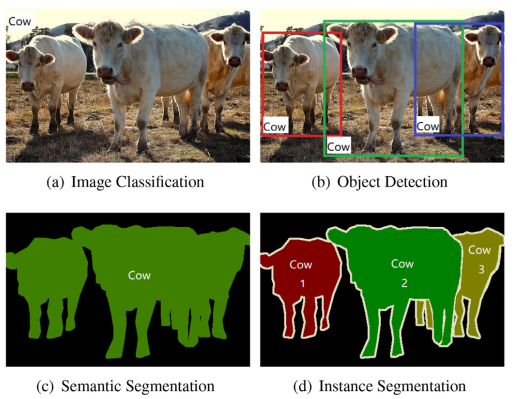
\includegraphics[width=0.8\textwidth]{object_detection}
  \caption{Detección, clasificación y segmentación. \cite{2019arXiv190803673W}}
  \label{fig:object-detection}
\end{figure}



\section{Dos pasos o basados en RCNN}
El problema de detección se divide en dos etapas: una generación de propuestas y la realización de predicciones sobre estas propuestas. Como paradigmas de detección, destacan la familia \emph{R-CNN} y los que se encuentran basados en esta.\newline

Esta familia surge en noviembre de 2013 con \emph{R-CNN} \cite{2013arXiv1311.2524G} que utiliza Selective Search \cite{Selective Search for object recognition} para generar 2000 bbox de propuestas que son redimensionadas para coincidir con las dimensiones de entrada una CNN pre-entrenada. Esta CNN debe volver a entrenarse, extrayéndole la última capa y añadiéndole una \emph{máquina de vectores de soporte(SVM)} con las categorías originales más una nueva clase llamada "fondo" que engloba a todas las propuestas que no pertenecen a ninguna categoría. Finalmente, las propuestas clasificadas son combinadas a través de un modelo de regresión lineal para así obtener una bbox con mejor ajuste y precisión.\newline

La principal diferencia que introduce \emph{Fast R-CNN} \cite{2015arXiv150408083G} reside en que, en lugar de pasar por la CNN todas las propuestas de Selective Search, nuestra CNN recibe como entrada la imagen completa reduciendo el coste computacional al analizar una única vez las zonas de solapamiento entre propuestas. Además, las propuestas dejan de ser escaladas para coincidir con una determinada dimensión y se introduce en una capa especial llamada \emph{Region of Interest Pooling Layer (RoI pooling)} que extrae un vector de longitud fija que será la entrada de las siguientes ramas. A continuación, el modelo se divide en dos ramas: un clasificador SoftMax y un modelo de regresión que calcula las bbox. \newline

\begin{figure}[htpb]
  \centering
  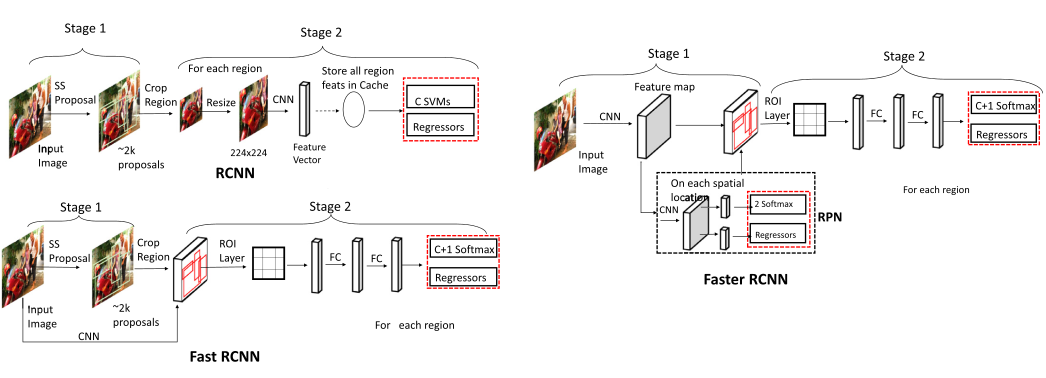
\includegraphics[width=1\textwidth]{rcnn}
  \caption{Comparativa de algunos modelos de la familia R-CNN. \cite{2019arXiv190803673W}}
  \label{fig:r-cnn}
\end{figure}

En \emph{Faster R-CNN} \cite{2015arXiv150601497R} se sustituye Selective Search por una red neuronal de generación propuestas, conocida como \emph{anchor boxes}, que no sólo reduce el tiempo de cómputo de la generación de propuestas sino que aporta un menor número de propuestas con mayor calidad y precisión. Un buen apunte de la red de generación de propuestas, es que esta no es pre-entrenada antes de ser añadido al modelo sino que aprende de forma conjunta con toda la red.\newline

La última mejora de esta familia viene representada por \emph{Mask R-CNN} \cite{2017arXiv170306870H} que sustituye la capa RoI pooling introducida en el modelo Fast R-CNN por una RoI alignment que retiene más información de las características obtenidas por la CNN compartiendo la misma estructura de entrada y salida de datos con la RoI pooling. Mask R-CNN aprovecha esto para realizar predicciones del tipo pixel level con mayor precisión a través de una interpolación bilineal que se ejecuta paralelamente con las capas totalmente conectadas de los modelos anteriores. Así, en el mismo punto que sus predecesores eran divididos en tres ramas independientes, Mask R-CNN se divide en tres ramas: un clasificador SoftMax, un regresor de bbox y un otro regresor de pixel level.\newline

Mencionar Mesh R-CNN
https://arxiv.org/abs/1906.02739\newline
Mencionar R-FCN
https://arxiv.org/pdf/1605.06409.pdf\newline
Libra R-CNN
https://arxiv.org/pdf/1904.02701.pdf
\section{Un paso o basados en YOLO}
Estos modelos destacan por no hacer una separación directa de la generación de propuestas y la predicción de estas. Destaca \emph{YOLO} y sus sucesivas mejoras, así como los múltiples algoritmos basados en ellas, pero existen muchos más modelos que pueden ser identificados con esta estructura.\newline

En junio de 2015 aparece \emph{You Only Look Once (YOLO)} \cite{2015arXiv150602640R}, un nuevo algoritmo que pretende realizar al mismo tiempo la generación de propuestas y la clasificación de estas, buscando así una mayor eficiencia computacional. Para ello, tras redimensionar la imagen en 448x448 píxeles, el algoritmo divide la imagen en una cuadrícula cuyas celdas se encargan de realizar un número fijo de propuestas indicando en cada una de ellas la probabilidad que tiene de ser un objeto, la bbox en la que se encuentra y la probabilidad de pertenecer a cada una de las clases de objetos de las que disponemos. Finalmente, descarta aquellas propuestas con baja probabilidad de ser un objeto y utiliza un algoritmo de \emph{non-max supression} \cite{2017arXiv170404503B} que unifica y combina las bbox con las máximas áreas compartidas.\newline

Buscando una mejora de la predicción pero sin perder el enfoque de la velocidad, surge \emph{YOLO9000} o \emph{YOLOv2} \cite{2016arXiv161208242R} que sigue la misma estructura que su predecesor pero sustituyendo algunos fragmentos por otros con mayor rendimiento. YOLOv2 redimensiona la imagen original a 416x416 píxeles y sustituye las capas totalmente conectadas que utilizaba para la generación de propuestas por un modelo de \emph{anchor boxes} \cite{2015arXiv150601497R} junto con otros cambios menores.\newline

La siguiente versión \emph{YOLOv3} \cite{2018arXiv180402767R} decide  no darle tanta importancia a la velocidad y centrarse en solucionar los problemas de detección presentados por sus antecesores. Mientras que YOLOv2 utiliza una arquitectura con 30 capas, YOLOv3 utiliza 106 capas totalmente convolucionadas e introduce la utilización de \emph{residual blocks}, \emph{skip connections} y \emph{upsampling}. Esta nueva arquitectura, realiza la detección de objetos en tres escalas distintas en diferentes profundidades de la red Darknet-53 y utilizando una estructura piramidal \cite{2016arXiv161203144L} para comunicar la detección entre las diferentes escalas.\newline

Mencionar YOLOv4
https://arxiv.org/pdf/2004.10934.pdf\newline

Feature Pyramid Networks
https://arxiv.org/pdf/1612.03144.pdf

\section{Non-local Neural Networks}

En \cite{DBLP:journals/corr/abs-1711-07971} se introduce el concepto de \emph{Non-local Neural Networks} que plantea un modelo de \emph{Feature Pyramid Network} para extraer las características de un clasificador a distintos niveles de profundidad y utilizarlas para segmentar semánticamente la imagen. \ref{fig:object_detection}\newline

FIXME: Insertar imagen del modelo genérico

Podemos distinguir tres tipos de componentes principales: clasificador, bloque no local o \emph{non-local block} y bloque de fusión o \emph{fuse up block}. Lo que más destaca de estas estructuras son los non-local block utilizados para extraer las características puesto que, en lugar obtenerlas utilizando de forma recurrente convoluciones en pequeñas áreas, comprueban las relaciones entre los datos con una única operación que, además, comprueba la afinidad con los datos más distantes.\newline

A continuación, nos centraremos en los non-local block, definiendo las clase de funciones que los forman y demostrando algunas de sus propiedades que garantizarán su correcto funcionamiento. Seguidamente, mostraremos algunos ejemplos y cómo podemos configurar nuestra propia red según nuestras necesidades.n\newline

\subsection{Non-local operation}

%\begin{definicion}
%Sea $X$ un espacio topológico, $Y$ un conjunto, $F(X)$ un espacio de funciones que contiene a todas las funciones cuyo dominio sea $X$ y $G(Y)$ otro espacio de funciones que contiene todas las funciones con dominio $Y$. Un operador $A:F(X)\to G(Y)$ se dice que es local si para todo $y\in Y$ existe un $x\in X$ tal que $Au(y)=Av(y)$ para todas las funciones $u,v\in F(X)$ que son equivalentes a $x$.
%\end{definicion}
\begin{definicion}
 Sea $x=(x_1,...,x_D)\in \R^D$ una señal de entrada, $u:\R \times \R \to \R$ un producto escalar, $v:\R \to \R$ y $C_x\in R$ una constante.  Se define una operación no local genérica o \emph{generic non-local operation} en una red neuronal profunda $f:\R^D \to \R^D$ con $f(x)=(f(x_1),...,f(x_D))$ donde:

 $$f(x_i)=\frac{1}{C_x}\sum_{\j=1}^{D} u(x_i,x_j)v(x_j) \; \;  \forall i=1,...,D$$
\end{definicion}

 En este contexto, $v$ será una representación de la señal de entrada en la posición $j$, $u$ representará una relación, por ejemplo la afinidad, entre los $i$ y $j$. La operación recibe este nombre debido a que considera todas las posiciones de la imagen para calcular el valor del filtro en la posición $i$ distinguiéndose así de una operación convolucional que se centraría en un rango \emph{local} de posiciones.% ($i-1\leq j \leq i+1$ en el caso de tener una convolución de núcleo de tamaño $3$).

Proseguiremos enunciando varios ejemplos de funciones que pertenezcan a dicha definición para mostrar la diversidad que podemos elegir a la hora de implementar un modelo que siga esta estructura. Por simplicidad, consideraremos que $v(x_j)=W_v x_j$ donde $W_v$ es una matriz de pesos que tiene que ser aprendida, siendo esta fácilmente implementable como una convolución de núcleo de tamaño $1$.

\begin{enumerate}
\item \emph{Gaussiana} $u(x_i,x_j)=e^{x_i^T x_j}$ y $C(x)= \sum_{j=1}^D u(x_i,x_j)$.
\item \emph{Embedded Gaussian} $u(x_i,x_j)=e^{\phi(x_i)^T,\theta(x_j)}$ donde $\phi(x_i)=W_\phi x_i$ y $\theta(x_j)=W_\theta x_j$ son dos inmersiones y  $C(x)= \sum_{j=1}^D u(x_i,x_j)$. Nótese que el módulo \emph{self-attention} es un caso particular de este ejemplo.
\item \emph{Dot-product similarity} $u(x_i,x_j)=\phi(x_i)^T \theta(x_j)$ donde $\phi(x_i)=W_\phi x_i$ y $\theta(x_j)=W_\theta x_j$ son dos inmersiones y $C(x)=D$.
\item \emph{Non-local means} \cite{}
% ¿Concatenacion?
\end{enumerate}

FIXME: Insertar definiciones básicas utilizadas en el enunciado

Sea $V$ un campo aleatorio (random field) y los datos de entrada $v$ una realización de $V$. Sea $Z$ una secuencia de variables aleatorias con $Z_i=\{X_i,Y_i\}$ con $Y_i=V(i)$ es real valuada y $X_i=V(I\backslash \{i\}) \R^p$ valuada donde $I$ representa el conjunto de posiciones. Una operación no local genérica será un estimador de la esperanza condicionada $E[Y_i|X_i=v(I\backslash{i})]$.

\begin{teorema}
Sea $Z={V(N_i\newline{i},V(i)}_{i\ge 1}$ un proceso estocástico estrictamente estacionario y mezclado \emph{strictly stationary and mixing process}. Sea $f^n$ una operación no local genérica aplicada a la secuencia $Z_n=\{V(N_i\backslash\{i\},V(i)\}_{i=1}^n$. Entonces, $$ |f^n(j)-[Y_j|X_j=v(I\backslash \{j\})]| \to 0 \; a.s \;  \forall j \in{1,...,n}$$.
\end{teorema}

En un contexto más general, la demostración se puede encontrar en \cite{A non local algorithm for image denoising}


\subsection{Non-local block}
Finalmente, el bloque non-local es de la forma: $$z_i=W_z f(x_i) + x_i$$, donde multiplicamos la función no local por un peso que será entrenado por la red y le añadimos una conexión residual para evitar perder las características del modelo pre-entrenado en caso de que $W_z$ comience siendo inicializado como $0$.

FIXME: Añadir más ventajas de la conexión residual.
